\section{Teedy Gideon Manik(1174038)}
\subsection{Point Polyline dan Polygon}
\begin{enumerate}
	\item 
	\lstinputlisting{src/1/1174038/1.py}
	\begin{figure}[H]
		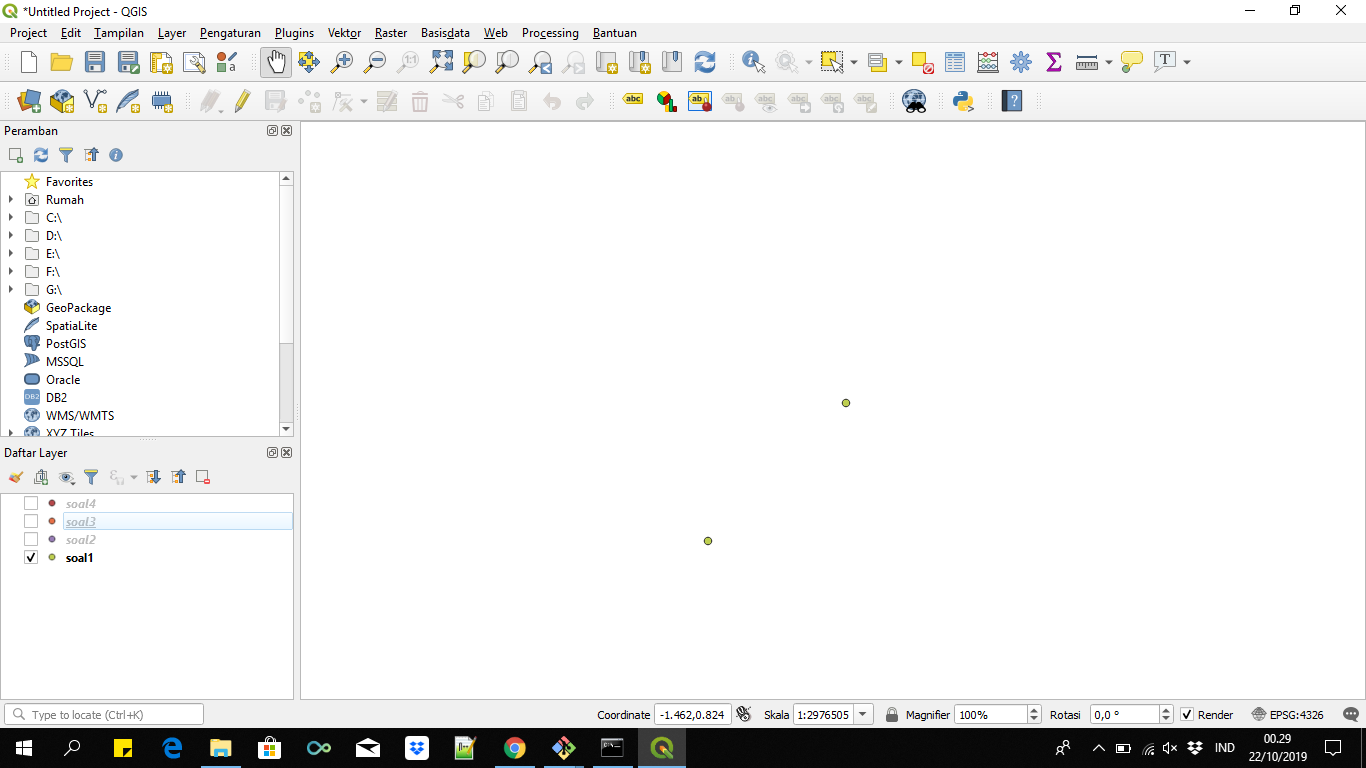
\includegraphics[width=12cm]{figures/1174038/1.PNG}
		\centering
		\caption{Point}
	\end{figure}
	
	\item 
	\lstinputlisting{src/1/1174038/2.py}
	\begin{figure}[H]
		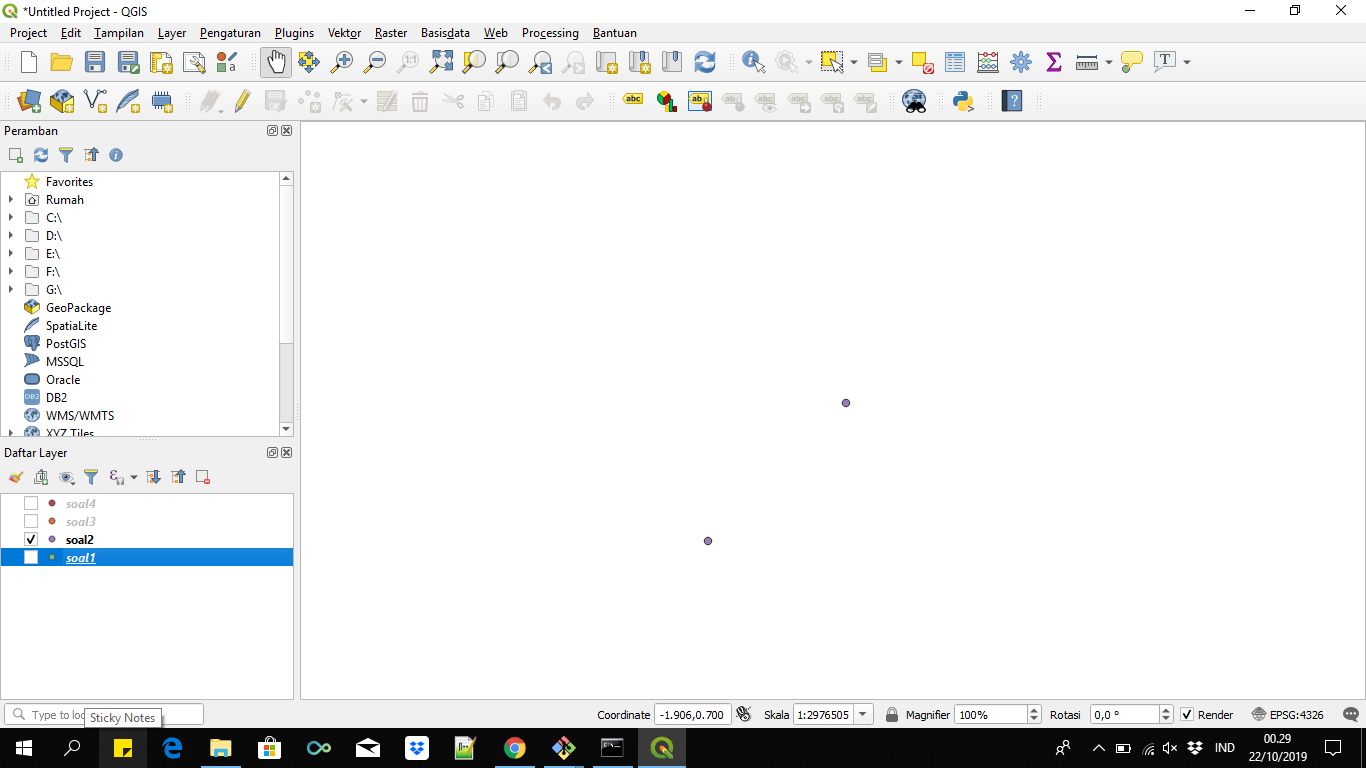
\includegraphics[width=12cm]{figures/1174038/2.PNG}
		\centering
		\caption{Point}
	\end{figure}
	
	\item 
	\lstinputlisting{src/1/1174038/3.py}
	\begin{figure}[H]
		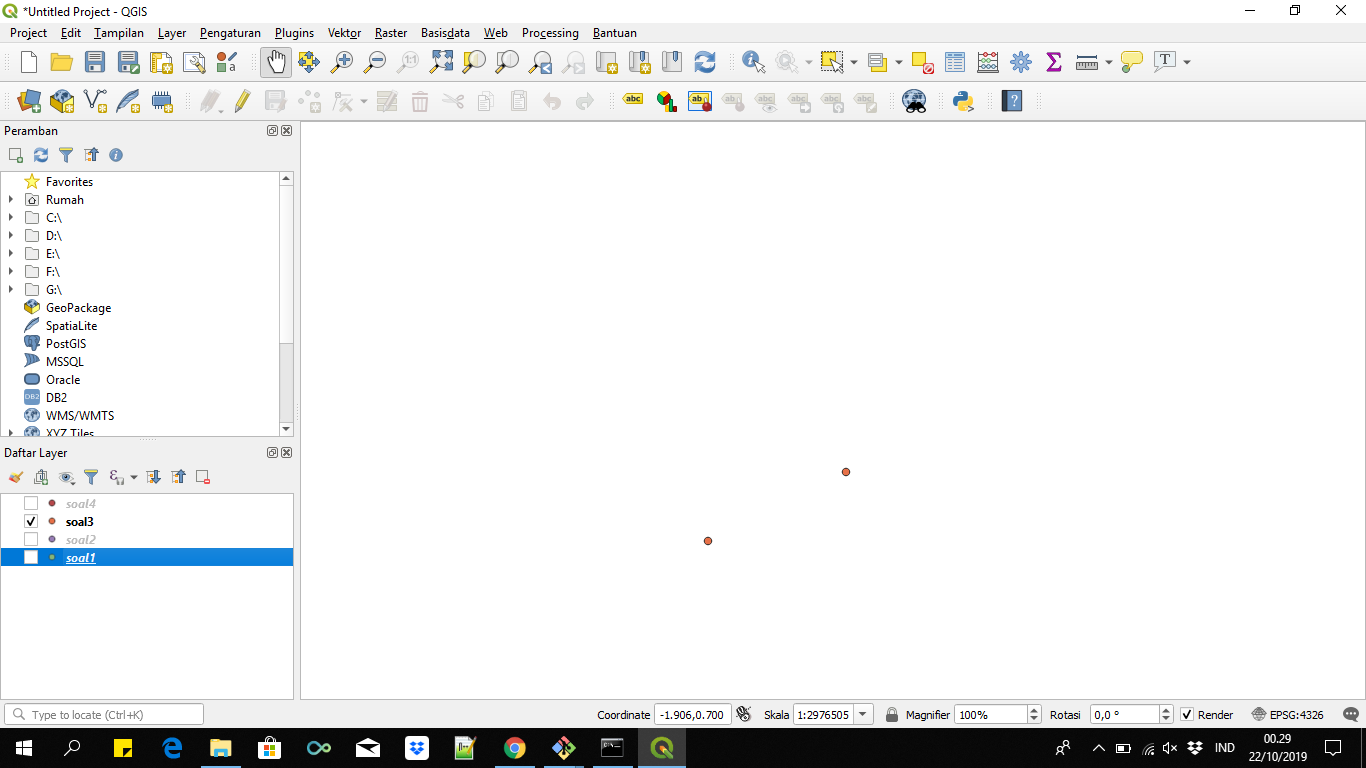
\includegraphics[width=12cm]{figures/1174038/3.PNG}
		\centering
		\caption{Point}
	\end{figure}
	
	\item 
	\lstinputlisting{src/1/1174038/4.py}
	\begin{figure}[H]
		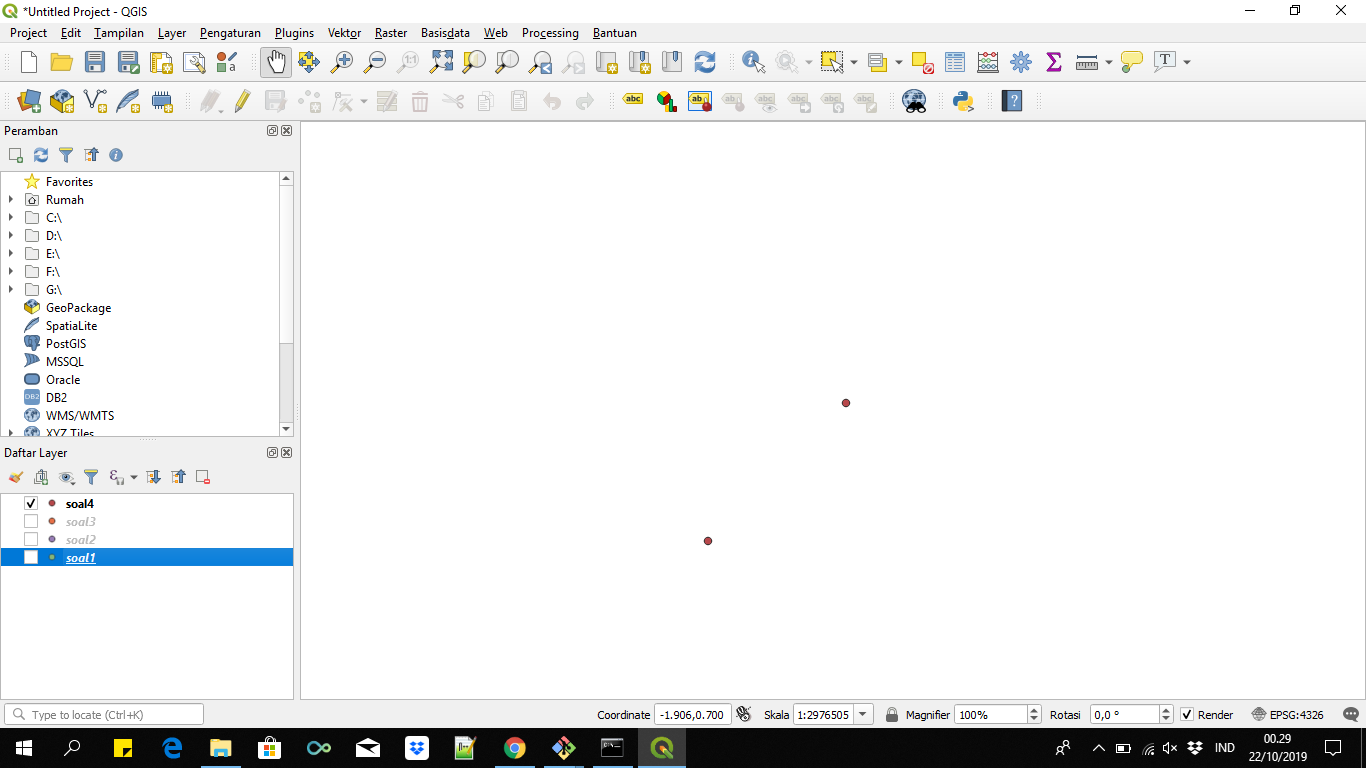
\includegraphics[width=12cm]{figures/1174038/4.PNG}
		\centering
		\caption{Point}
	\end{figure}
	
	\item 
	\lstinputlisting{src/1/1174038/5.py}
	\begin{figure}[H]
		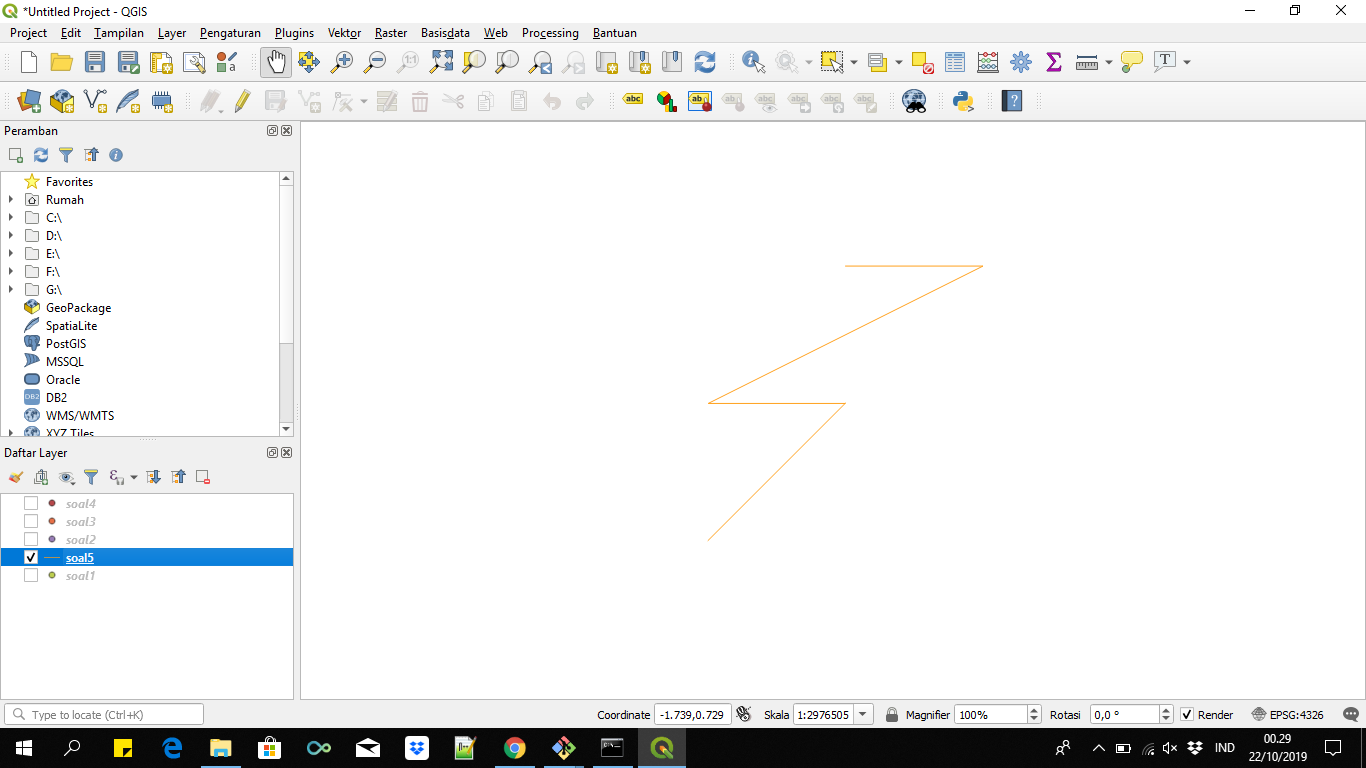
\includegraphics[width=12cm]{figures/1174038/5.PNG}
		\centering
		\caption{Polyline}
	\end{figure}
	
	\item 
	\lstinputlisting{src/1/1174038/6.py}
	\begin{figure}[H]
		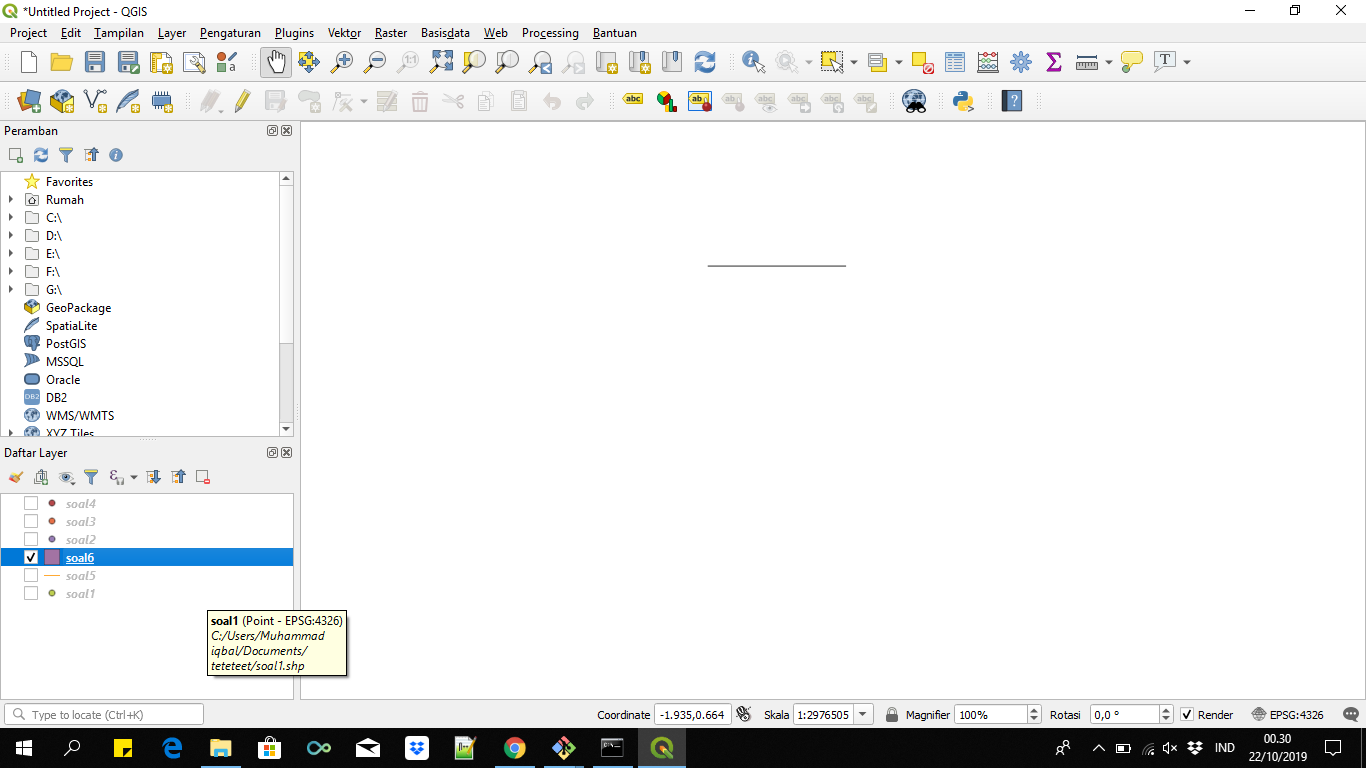
\includegraphics[width=12cm]{figures/1174038/6.PNG}
		\centering
		\caption{Poligon}
	\end{figure}
	
	\item 
	\lstinputlisting{src/1/1174038/7.py}
	\begin{figure}[H]
		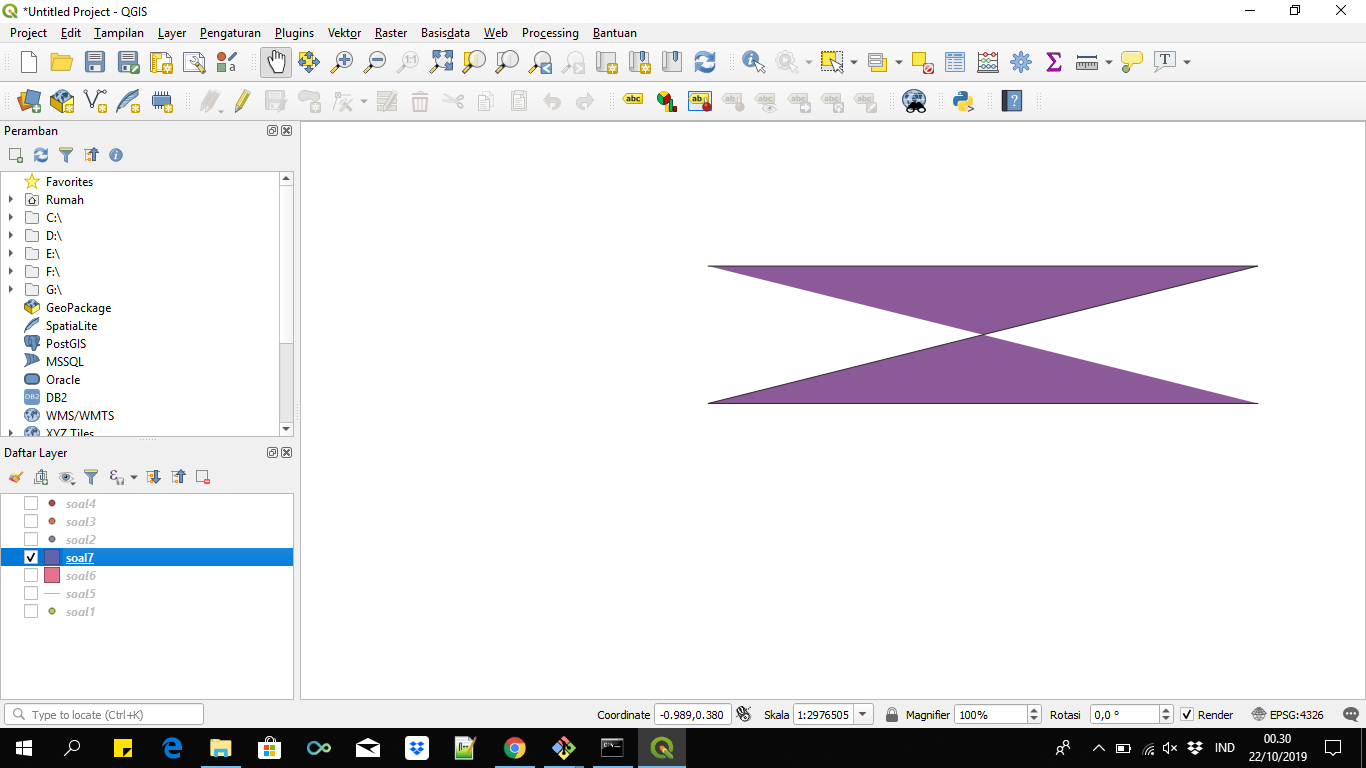
\includegraphics[width=12cm]{figures/1174038/7.PNG}
		\centering
		\caption{Polygon}
	\end{figure}
	
	\item 
	\lstinputlisting{src/1/1174038/8.py}
	\begin{figure}[H]
		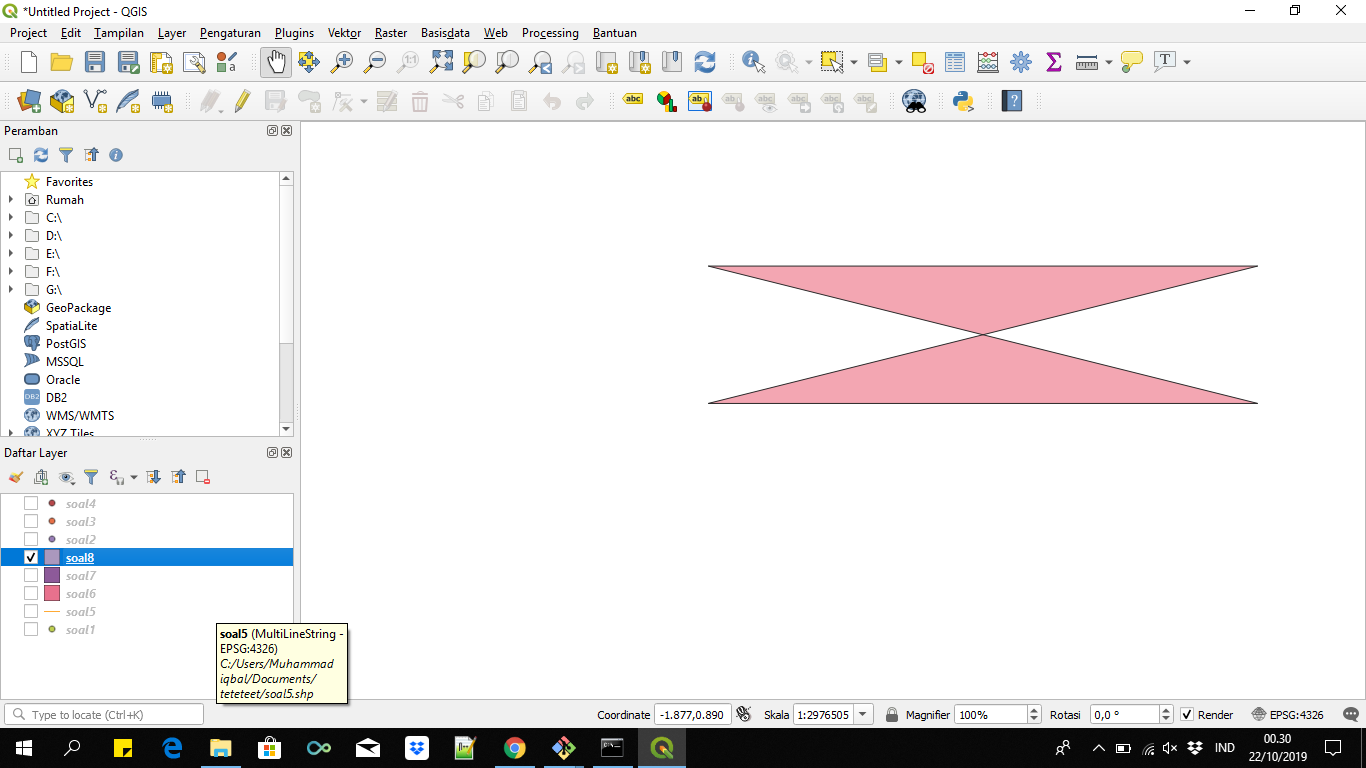
\includegraphics[width=12cm]{figures/1174038/8.PNG}
		\centering
		\caption{Polygon}
	\end{figure}
	
	\item 
	\lstinputlisting{src/1/1174038/9.py}
	\begin{figure}[H]
		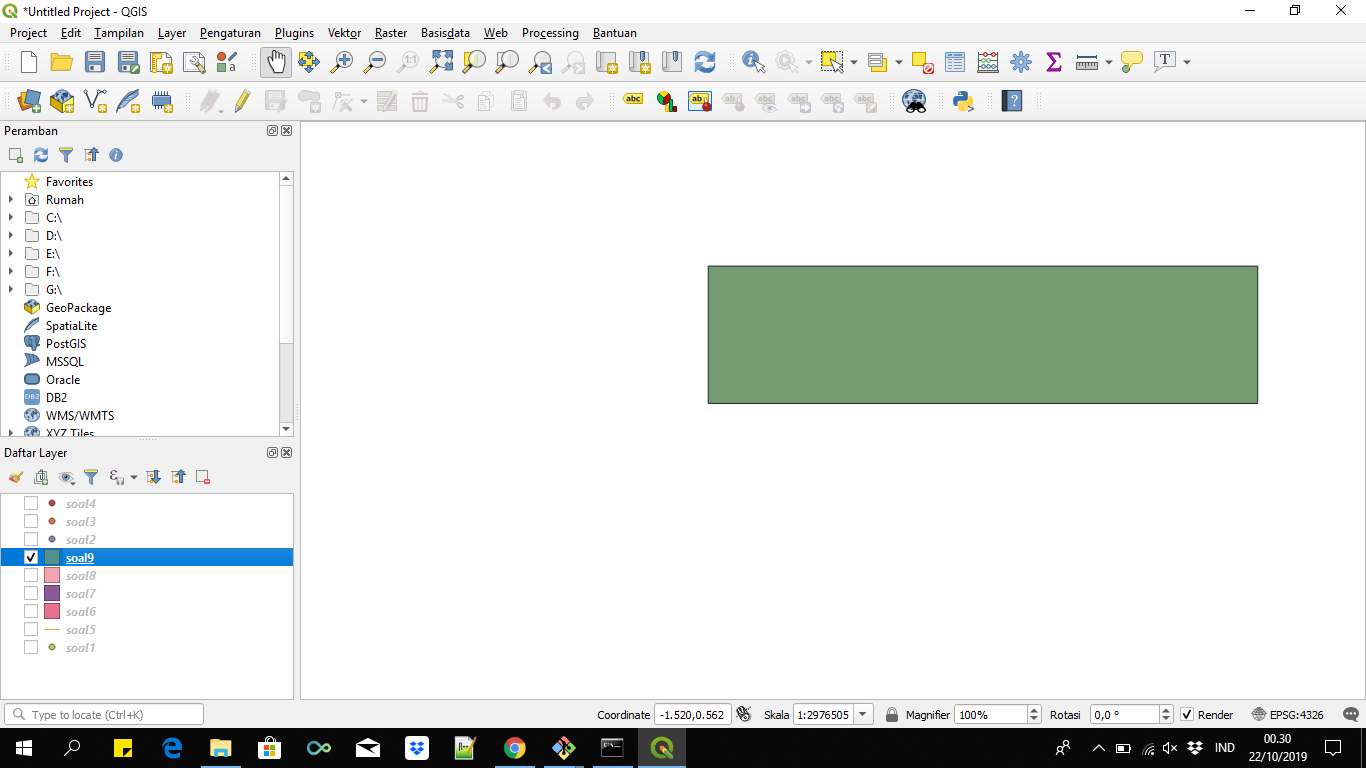
\includegraphics[width=12cm]{figures/1174038/9.PNG}
		\centering
		\caption{Polygon}
	\end{figure}
	
	\item 
	\lstinputlisting{src/1/1174038/10.py}
	\begin{figure}[H]
		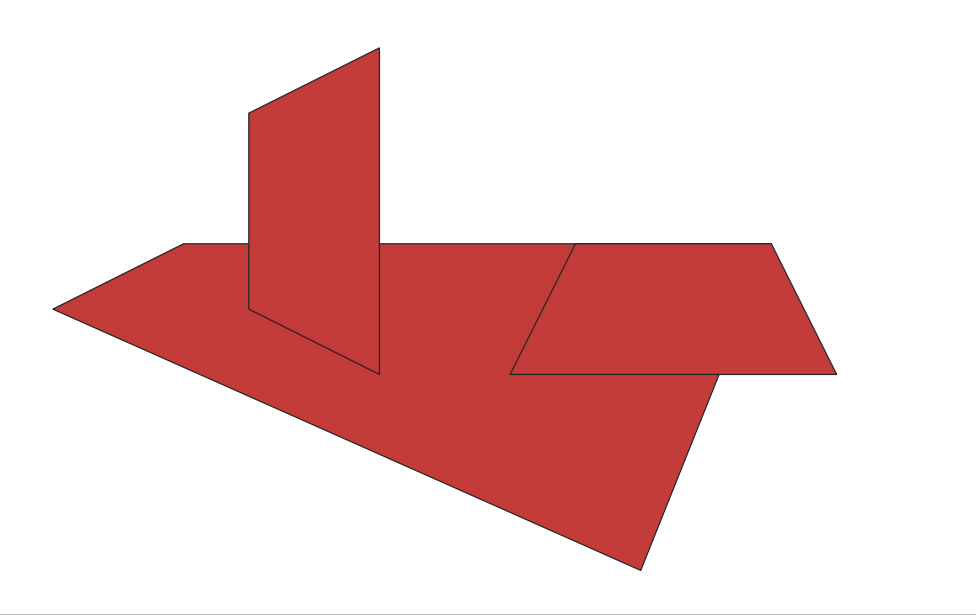
\includegraphics[width=12cm]{figures/1174038/10.PNG}
		\centering
		\caption{Hasil mod saya yaitu 6 jadi yang saya kerjakan Trapesium yang berjumlah 3, Polygon}
	\end{figure}	
\end{enumerate}

\subsection{Link}
\href{https://youtu.be/-kGuJYmKhJY}{Youtube! JANGAN LUPA SESKREB!!}